%---------------------导言区---------------------------%
\documentclass[12pt,a4paper,UTF8]{ctexart}
	%10pt：正文字体为12pt，缺省为10pt；各层级字体大小会根据正文字体自动调整
	%a4paper：纸张大小a4；
	%UTF8：中文要求
\usepackage{geometry}%用于设置上下左右页边距
	\geometry{left=2.5cm,right=2.5cm,top=3.2cm,bottom=2.8cm}
\usepackage{xeCJK}
\usepackage{amsmath}
\usepackage{paralist}
\usepackage{enumerate}
\usepackage{booktabs}
\usepackage{multirow}
\usepackage{graphicx}
\usepackage{subfig}
\usepackage{setspace}
\usepackage{listings}
\usepackage{lastpage}
\usepackage{hyperref}
\usepackage{pdfpages}

%xeCJK：中文字体（如楷体，作者和机构需要用到）的设置
	%amsmath：数学公式
	%paralist，enumerate：自定义项目符号
	%booktabs：三线图，论文常用的表格风格
	%multirow：复杂表格
	%graphicx，float: 插入图片
	%subfig：并排排版图片、竖向排版图片
	%setspace：设置行间距等功能
	\setlength{\parindent}{2em}%正文首行缩进两个汉字
	%listings:用于排版各种代码；比如matlab的代码
	\lstset{language=Matlab}%matlab代码
	%lastpage:获取总页数;
	%hyperref:超链接,和lastpage搭配.
\usepackage{fancyhdr}
	%fancyhdr：一个很强大的宏包，用于自定义设计页面风格并命名以供调用。
	\pagestyle{fancy}
	\rhead{气体放电和等离子体诊断实验}
	\lhead{近代物理实验~~~实验报告}
	\cfoot{Page \thepage/\pageref{LastPage}}  %当前页\总页数
	\rfoot{\today}
		%分别是右页眉、左页眉、中页脚、右页脚
	\renewcommand{\headrulewidth}{0.4pt}
	\renewcommand{\theenumi}{(\arabic{enumi})}

%%%%%%%%%%%%%%%%%%%%%%%%%%%%%%%%%%%%%%%%%%%%%%%%%%%%%%%%%%
%%%%%%%%%%%%%%%%%%%%%%%%%正文开始%%%%%%%%%%%%%%%%%%%%%%%%%%
%%%%%%%%%%%%%%%%%%%%%%%%%%%%%%%%%%%%%%%%%%%%%%%%%%%%%%%%%%

\begin{document}

%%begin-------------------标题与信息-----------------------%%

%%标题
\begin{center}
\LARGE\textbf{气体放电和等离子体诊断实验}
\end{center}

%%信息
\begin{doublespacing}
	%doublespacing：手动两倍行距
	\begin{tabular}{lr}
	 & \\
	 {实验人姓名：徐殊行~23343071} & {合作者姓名：王志超~23343062}\\
	 {实验时间：2025年4月18日/4月25日} & {室温：30$^{\circ}$C~相对湿度：60\%}
	
	\end{tabular}
\end{doublespacing}

%%-------------------中英文摘要-----------------------%%
\begin{abstract}
	气体放电作为近代物理和等离子体物理的重要基础现象，广泛应用于真空电子学、材料科学与航天技术等领域。\cite{yang_gasdischarge}
	本实验通过观察放电管内的气体放电现象，测量并分析放电管的V-I特性曲线，深入理解了气体导电与金属导电的本质区别。\cite{hu_electronics}
	实验进一步利用朗缪尔探针对辉光放电正柱区内的等离子体进行了诊断，测量了探针的I-V特性曲线，并由此计算得到了等离子体的空间电位、电子温度与等离子体密度。\cite{plasmart2004probe}
	通过实验操作与数据分析，掌握了正常辉光放电不同区域的物理特征及其形成机制，加深了对气体放电过程及等离子体基本性质的认识，为后续从事相关等离子体技术研究与应用奠定了实验基础。\cite{smartvacuum2017}
	
	\noindent \textbf{关键词：气体放电；辉光放电；V-I特性曲线；朗缪尔探针；等离子体诊断} 
		
\end{abstract}
	
\renewcommand{\abstractname}{Abstract}

\begin{abstract}
	Gas discharge, as a fundamental phenomenon in modern physics and plasma physics, finds wide applications in vacuum electronics, materials science, aerospace technology, and other fields.\cite{hiden2003probe}
	In this experiment, the gas discharge phenomena within a discharge tube were observed, and the V-I characteristic curve of the discharge tube was measured and analyzed, providing a deeper understanding of the essential differences between gas and metal conduction.\cite{smartprobe2002manual}
	Furthermore, Langmuir probe diagnostics were performed in the positive column region of the glow discharge to measure the I-V characteristic curve, from which the plasma space potential, electron temperature, and plasma density were calculated.\cite{plasmart2004probe}
	Through experimental operations and data analysis, the physical characteristics and formation mechanisms of different regions in normal glow discharge were mastered, enhancing the understanding of the gas discharge process and fundamental plasma properties, and laying a solid experimental foundation for future research and applications in plasma-related technologies.
	
	\noindent \textbf{Keywords: gas discharge~~ glow discharge~~ V-I characteristic curve~~ Langmuir probe~~ plasma diagnosis}
\end{abstract}

%%-------------------正文部分-----------------------%%

\subsection*{【实验目的】}

\begin{enumerate}[(1)]
	\item 学习气体放电的原理、物理图像。
	\item 掌握气体放电与等离子体诊断仪的使用方法。
	\item 测量气体放电的V-I特性曲线并分析不同阶段放电形式。
	\item 观察正常辉光放电的外型并解释现象。
	\item 了解空间电荷及等离子体，根据朗缪尔探针测量的I-V特性曲线计算电子温度、等离子体密度。
\end{enumerate}

\subsection*{【实验原理】}

\subsubsection*{1.气体放电的基本特点}


为了对气体放电的特性有概括性的认识，首先将气体放电与金属导电进行对比，分析两者的基本差别。

金属由组成晶格的正离子和在晶格中做热运动的自由电子组成。
在金属导电中，参与导电的只是自由电子（实际上是处于费米能级以上的自由电子）。
正离子只在其平衡位置附近震动，并不参与导电。

气体主要由中性的原子或分子组成，因此本身并不存在可以参与导电的带电粒子。
气体之所以能导电，是由于以下几方面原因：

\begin{itemize}
    \item 外界刺激产生载流子：自然界中的紫外线、宇宙射线、放射性粒子等，可以使气体分子电离，产生电子和正离子；
    辐射粒子撞击电极引起光电效应；
    加热气体产生热电子发射等。
    由此产生的载流子称为原始载流子。
    \item 内部相互作用产生载流子：已存在的电子和离子与气体分子碰撞，引发进一步电离或激发，从而产生新的载流子。
    由此产生的载流子称为次级载流子。


    通过近似自由电子模型，可以计算气体的电导率，其表达式为：

    \begin{equation}
        \sigma = \frac{n e^2 \lambda_e}{m_e C_e}
    \end{equation}

    其中，$n$为电子密度，$e$为电子电量，$\lambda_e$为电子平均自由程，$m_e$为电子质量，$C_e$为电子的平均速度。

    对于金属，$n$和$\lambda_e$在一定温度下基本恒定，因此其电导率也是定值；
    而对于气体，$n$和$\lambda_e$都随外界条件（如温度、电压、气压）变化，因此气体的电导率也是变化的。
    这是气体放电区别于金属导电的特点之一。

    宏观上，导电能力通过电阻描述，气体放电的伏安特性曲线呈复杂的曲线状，而金属导电的伏安特性曲线则是一条斜率恒定的直线。
    这是气体放电区别于金属导电的特点之二。

    \item 在金属导电中，能量转换主要是自由电子的动能转化为晶格振动能；
    而在气体放电中，载流子的能量不仅可以转化为热能，还可以引起激发、电离、辐射等非弹性过程。
    因此，气体放电的能量转换机制更加复杂。
    这是气体放电区别于金属导电的特点之三。

\end{itemize}

综上所述，气体放电相较于金属导电具有载流子种类多、载流子浓度变化大、伏安特性曲线复杂、能量转换形式多样等基本特点。

\subsubsection*{2.气体放电实验装置和现象}

气体放电的实验装置如图所示，整个过程在真空玻璃管中进行，该玻璃容器称为放电管\cite{dongbei1977vacuum,dongbei1981vacuum}。
真空度一般为几个托左右，管内安装有两个电极。
通过可变电阻$R$调节放电管两端的电压。
为测量放电电流，需在电路中串联微安表；测量电压时，在放电管两端并联伏特表。\cite{smartvacuum2017}

实验时，接通电源，通过调节限流电阻$R$，逐渐增大加在放电管两端的电压。
通过伏特表读取电压$U$，通过微安表读取电流$I$，从而记录气体放电的伏安特性曲线。

\begin{figure}[h!]
    \centering
    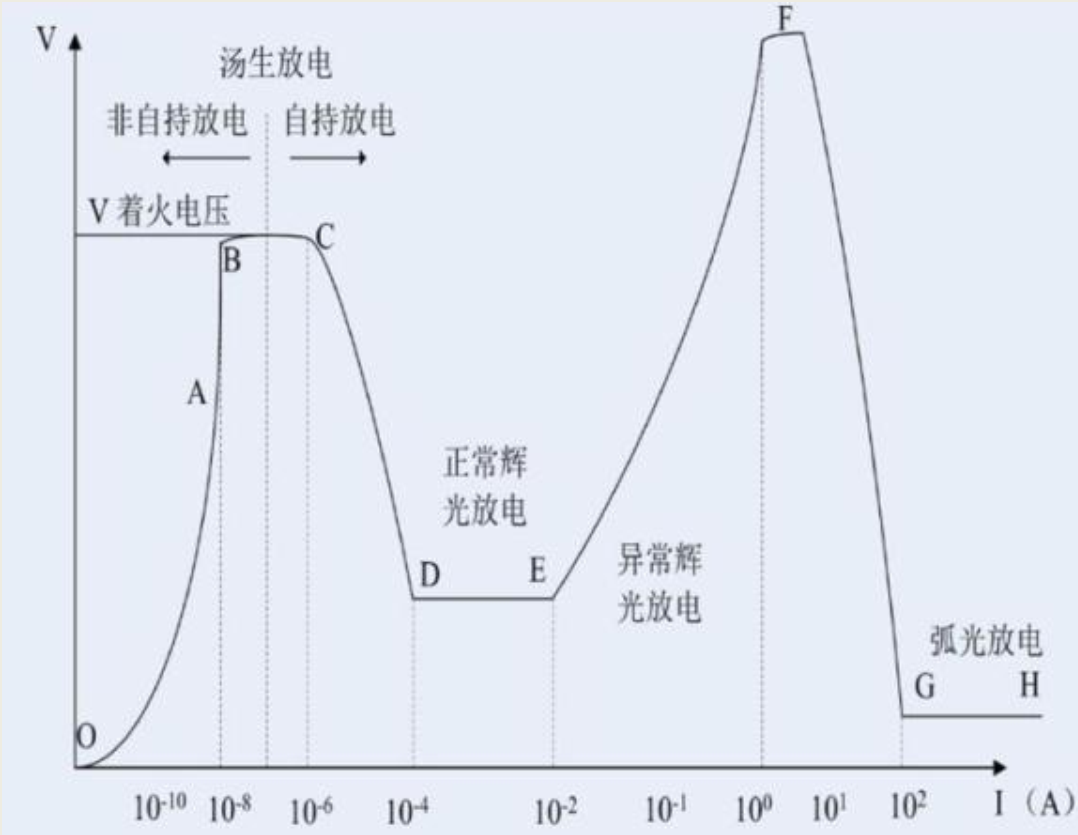
\includegraphics[width=0.8\textwidth]{VI.png}
    \caption{气体放电的V-I特性曲线}
\end{figure}

实验观察表明，放电电流值不同，放电现象表现出不同的阶段，具体如下\cite{smartvacuum2017,chen2003langmuir,yang_gasdischarge}：

\begin{enumerate}
    \item \textbf{汤生放电阶段}：初始时，在外界辐射（如高能光子）作用下，气体分子电离产生电子，这些电子进一步碰撞气体分子产生新的电子，形成自激过程。
    汤生放电受气体成分、电极材料等影响显著，放电不稳定，发出微弱光亮。
    
    \item \textbf{辉光放电阶段}：当自激过程足够强大，放电变为自持放电。
    破裂后电流增加而电压下降，放电进入辉光放电区，放电趋于稳定，阴极表面出现柔和的辉光。
    
    \item \textbf{正常辉光放电阶段}：在辉光放电中，随着电流增加，电压基本保持稳定，同时放电管内出现明暗相间的结构区域。
    此阶段应用于稳压器、霓虹灯等。
    
    \item \textbf{异常辉光放电阶段}：电流继续增加，电压也开始上升（接近线性），此阶段常应用于等离子体清洗、磁控溅射等工艺。
    
    \item \textbf{弧光放电阶段}：当电压达到峰值后，继续增加电流时，电压反而迅速下降至几十伏特并保持不变，电流急剧上升，电极表面发射大量电子，形成明亮的弧光。
    此阶段需采用水冷阴极，常用于电弧离子镀膜、真空熔炼等领域。
\end{enumerate}

本实验主要观察并测量正常辉光放电区域内气体放电的现象与特性，记录伏安特性曲线并结合放电外形图进行分析解释。

\subsubsection*{3.等离子体诊断}

在正常辉光放电的正柱区域，通过朗缪尔探针对等离子体性质进行测量和诊断。
实验中，将朗缪尔探针插入正柱区，测量其电流-电压（I-V）特性曲线，并据此分析以下等离子体参数：

\begin{itemize}
    \item \textbf{等离子体悬浮电位（$V_f$）}：探针电流$I=0$时探针的电位。
    \item \textbf{等离子体空间电位（$V_p$）}：对应电流饱和区域的探针电位。
    \item \textbf{电子温度（$T_e$）}：通过I-V曲线过渡区的对数变换（$\ln(I)$-$V$图）计算得出，斜率满足：
    \begin{equation}
        \text{slope} = \frac{e}{kT_e}
    \end{equation}
    其中$e$为元电荷，$k$为玻尔兹曼常数。
    \item \textbf{等离子体密度（$n_e$）}：根据电子饱和电流$I_{\text{sat}}$，利用公式估算：
    \begin{equation}
        I_{\text{sat}} = n_e e A \sqrt{\frac{kT_e}{2\pi m_e}}
    \end{equation}
    其中$A$为探针有效面积，$m_e$为电子质量。
\end{itemize}

朗缪尔探针通常由高熔点细金属丝制成（如钨丝、钼丝），针尖尺寸小于德拜长度，以尽量减小对等离子体本身的扰动。

\subsection*{【实验仪器】}
气体放电和等离子气体诊断实验仪

\subsection*{【实验内容】}
\cite{smartprobe2002manual}
\subsubsection*{1.气体放电}
\begin{itemize}
	\item 检查进气阀，气压微调阀
	\item 抽真空
	\item 充气、调节真空度
	\item 打开电压电源
	\item 测量并记录在四组不同压力下的气体放电的V-I特性曲线并分析不同阶段放电形式
	\item 观察正常辉光放电的外型并解释现象
	\item 实验结束后档位复原
\end{itemize}

\subsubsection*{2.等离子体诊断}
\begin{itemize}
	\item 检查进气阀，气压微调阀
	\item 抽真空
	\item 充气、调节真空度
	\item 打开电压电源
	\item 调节放电管的V-I特性曲线，使朗缪尔探针位于等离子体区（即正柱区）
	\item 选取合适的步长，测量等离子区的I-V特性曲线
	\item 读出等离子体悬浮电位、等离子体空间电位
	\item 计算出电子温度和等离子体密度
	\item 实验结束后档位复原
\end{itemize}

\subsection*{【实验过程和数据处分析处理】}
仔细阅读上述实验过程，并检查实验仪器完整可用之后我们开始实验。
我们主要检查的是电源的连接，设备是否接地，气阀连接是否正确等。

\textbf{在实验的第一周进行的是气体放电实验}

这里需要特别提到的是气阀的连接，因为在实验开始前，我们发现我们使用的设备上，气阀连接到了实验室的氦气源，放电管中是氦气环境。
而当天实验的其他小组的气阀是直接与空气联通的，放电管中是空气环境。
原因是我们组使用的设备在先前被用于其他的实验，而实验人员在使用完之后没有断开氦气的连接。
断开其连接之后我们便开始了正式实验。

\subsubsection*{1.调整真空度}

首先需要将气阀拧松，打开真空泵，开始抽真空。当真空度达到$5\mathrm{Pa}$时，我们开始调节气压微调旋钮，使放电管中地气压达到实验需要的不同数值。

\subsubsection*{2.测量气体放电的V-I特性曲线} 

调节完毕之后，我们开始测量气体放电的V-I特性曲线。
首先需要将总电压调节至$1050\mathrm{V}$左右，然后调节限流电阻，同时记录下电压和电流的数值，就可以得到气体放电的V-I特性曲线。

测量得到的曲线如下，其中x坐标轴采用了对数坐标。

\begin{figure}[h!]
    \centering
    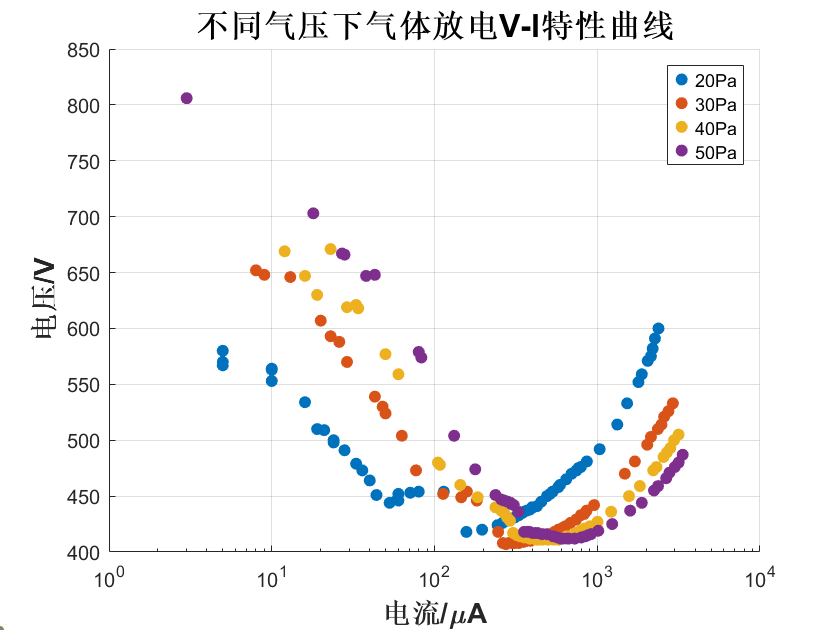
\includegraphics[width=0.8\textwidth]{气体放电VI.png}
    \caption{不同气压下气体放电V-I特性曲线}
\end{figure}

可见我们测量得到的曲线和理想中的曲线存在较大差异。
其中一个重要的原因是，我们使用的仪器对于电流的测量精度范围有限，我们无法测量$I<10^{-6}\mathrm{A}$或者$I>10^{-3}\mathrm{A}$的电流。
这导致我们无法观察到汤生放电阶段和弧光放电阶段。

不过从我们测量的数据图中还是能够观察到正常辉光放电阶段和异常辉光放电阶段，体现在测量曲线上，每一个气压下的曲线都存在一小段电流随电压增加而基本保持不变的区域。

\subsubsection*{3.观察辉光放电的实验现象}

在实验过程中，我们观察到了不同气压下辉光放电的现象。下图展示了四种不同气压条件下的辉光放电现象：
\begin{figure}[h!]
    \centering
    \subfloat[20Pa时的正常辉光放电]{
        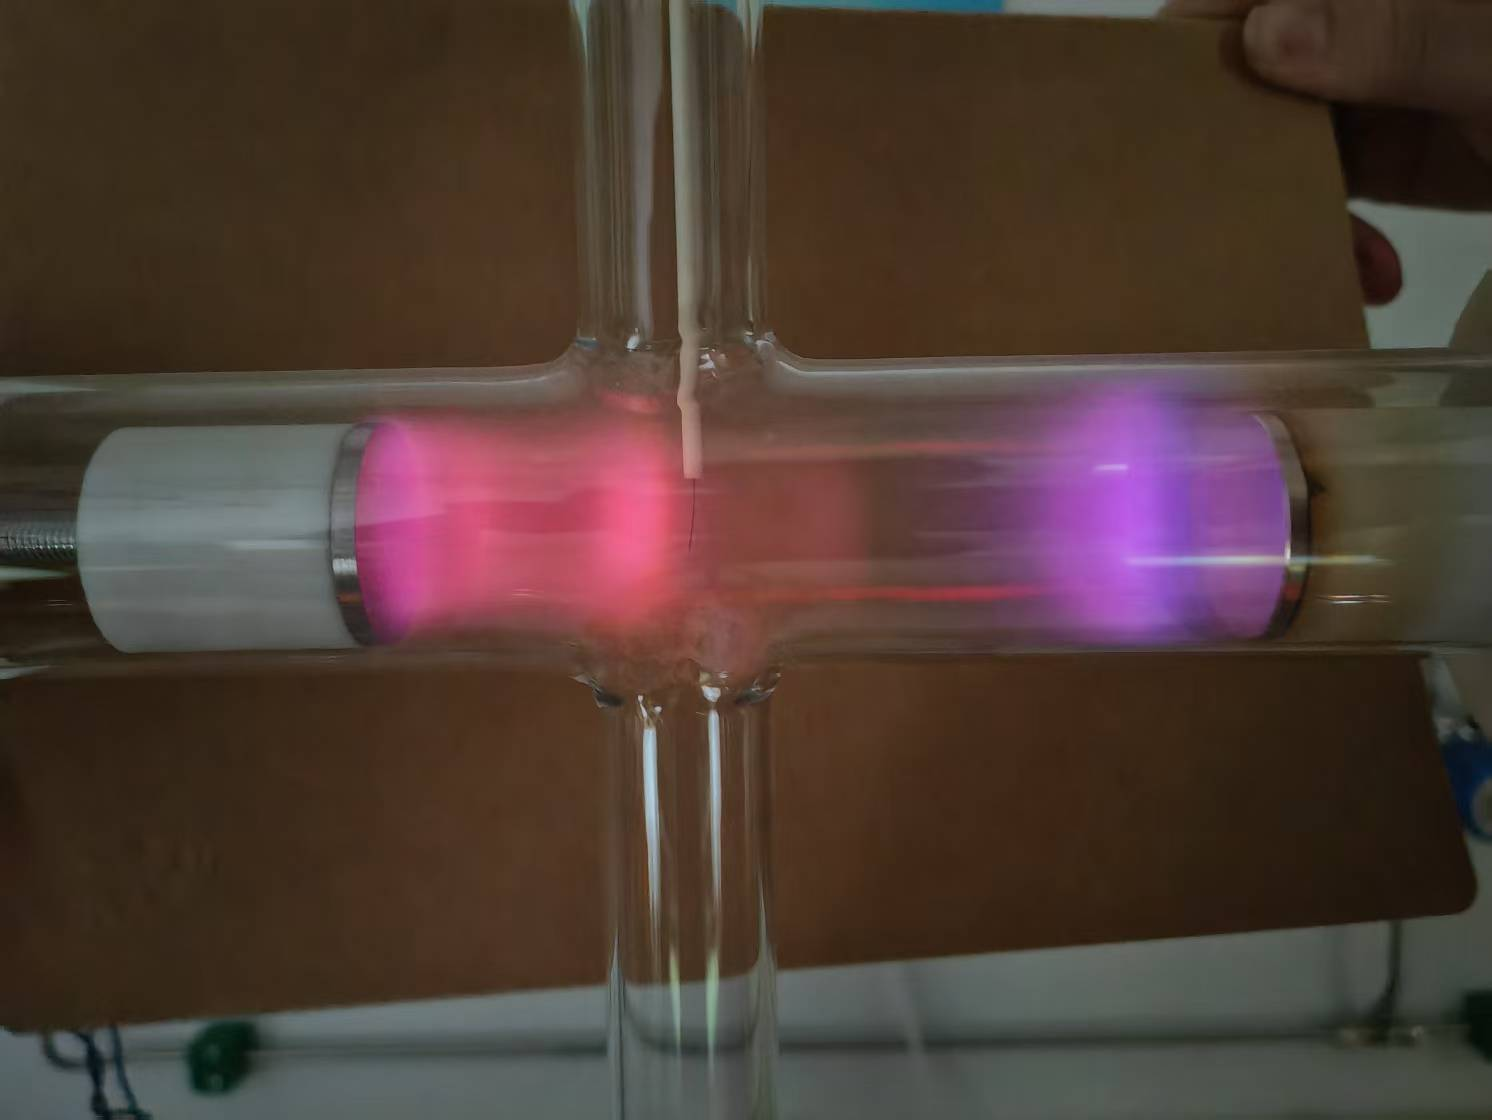
\includegraphics[width=0.3\textwidth]{20正常.jpg}
    }
    \subfloat[30Pa时的正常辉光放电]{
        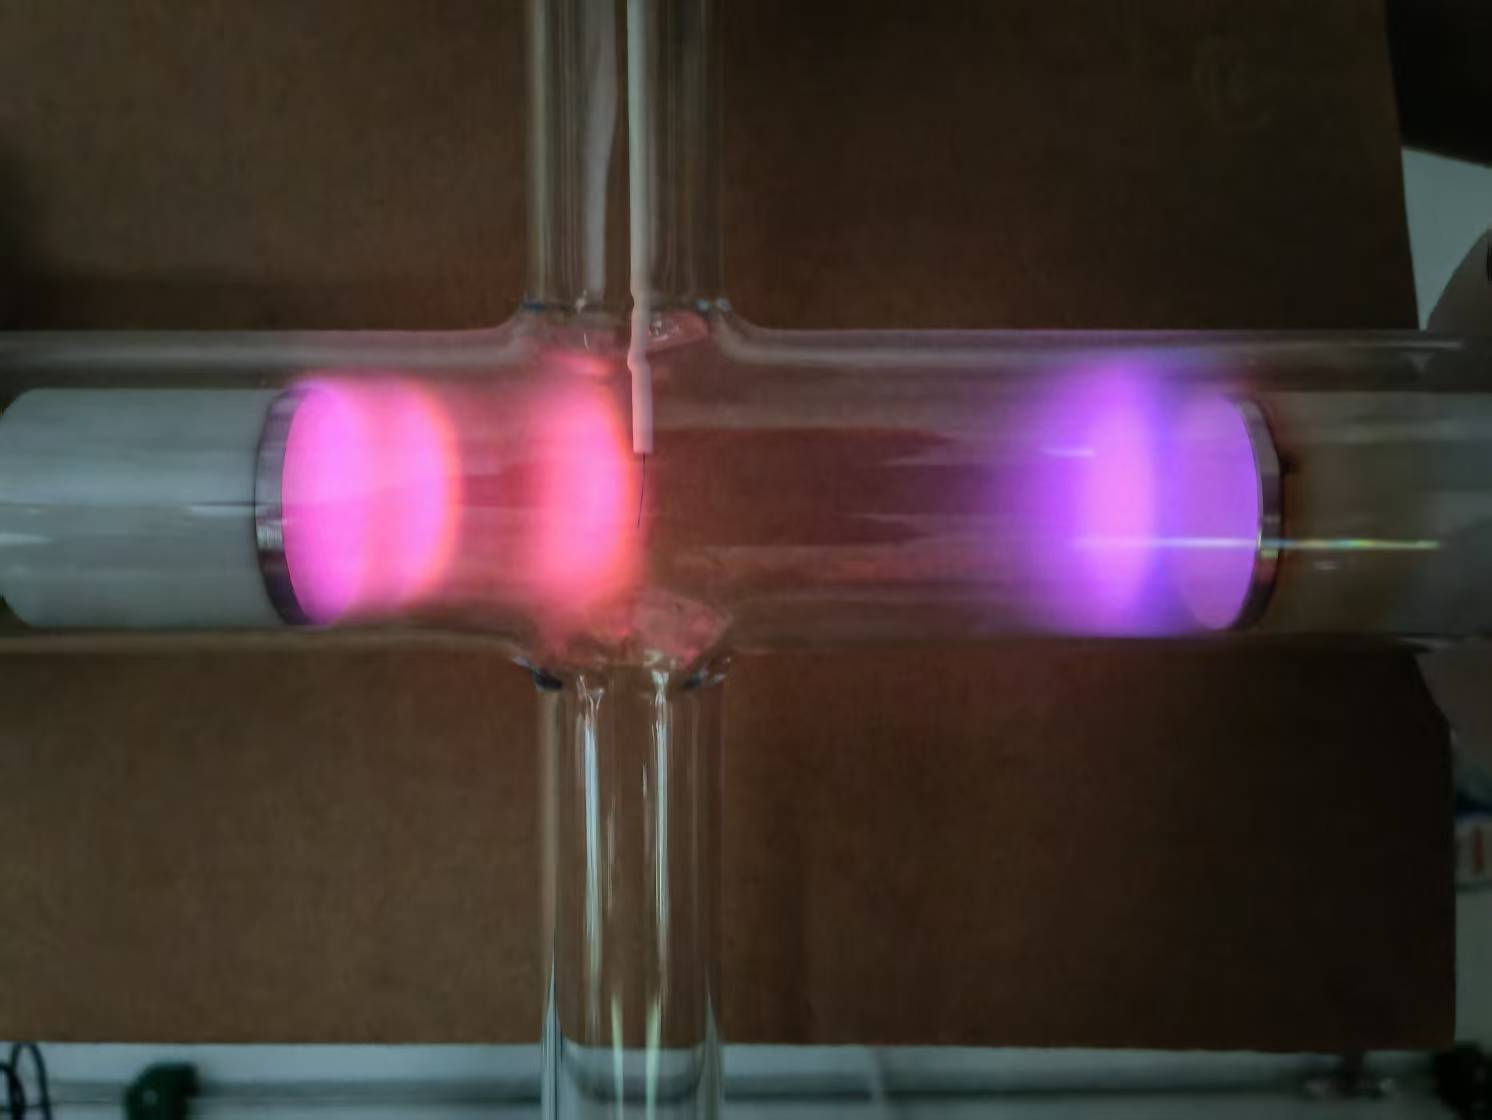
\includegraphics[width=0.3\textwidth]{30正常.jpg}
    }
    \subfloat[40Pa时的正常辉光放电]{
        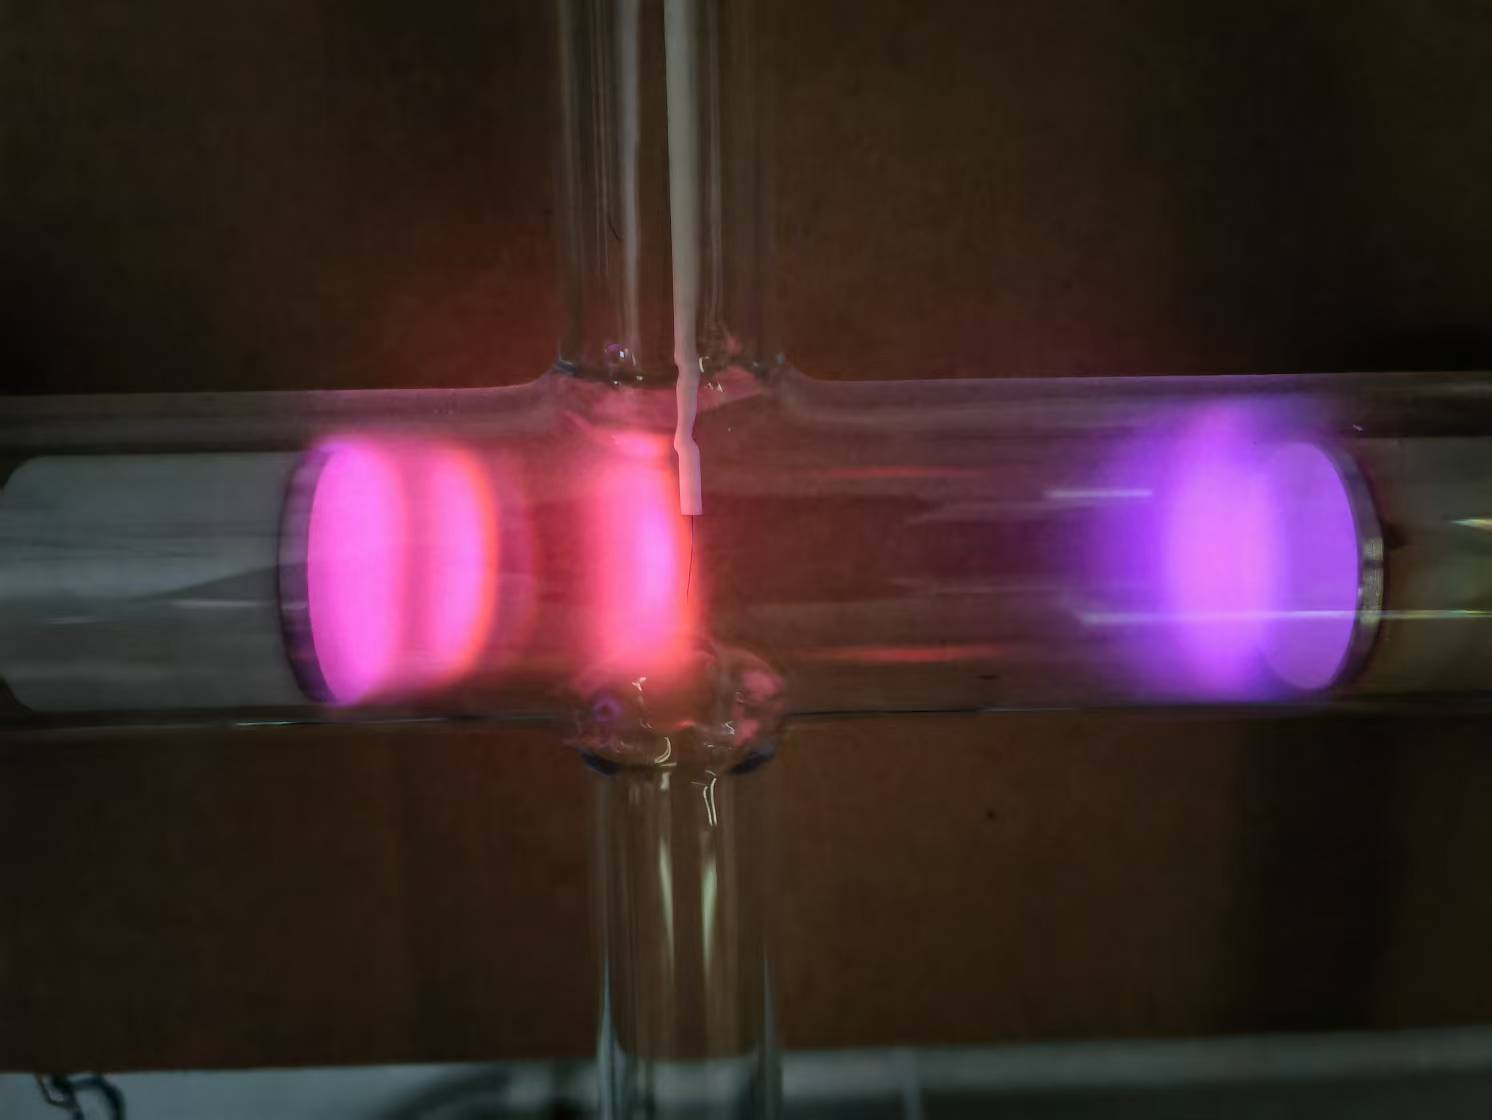
\includegraphics[width=0.3\textwidth]{40正常.jpg}
    }\\
    \subfloat[20Pa时的异常辉光放电]{
        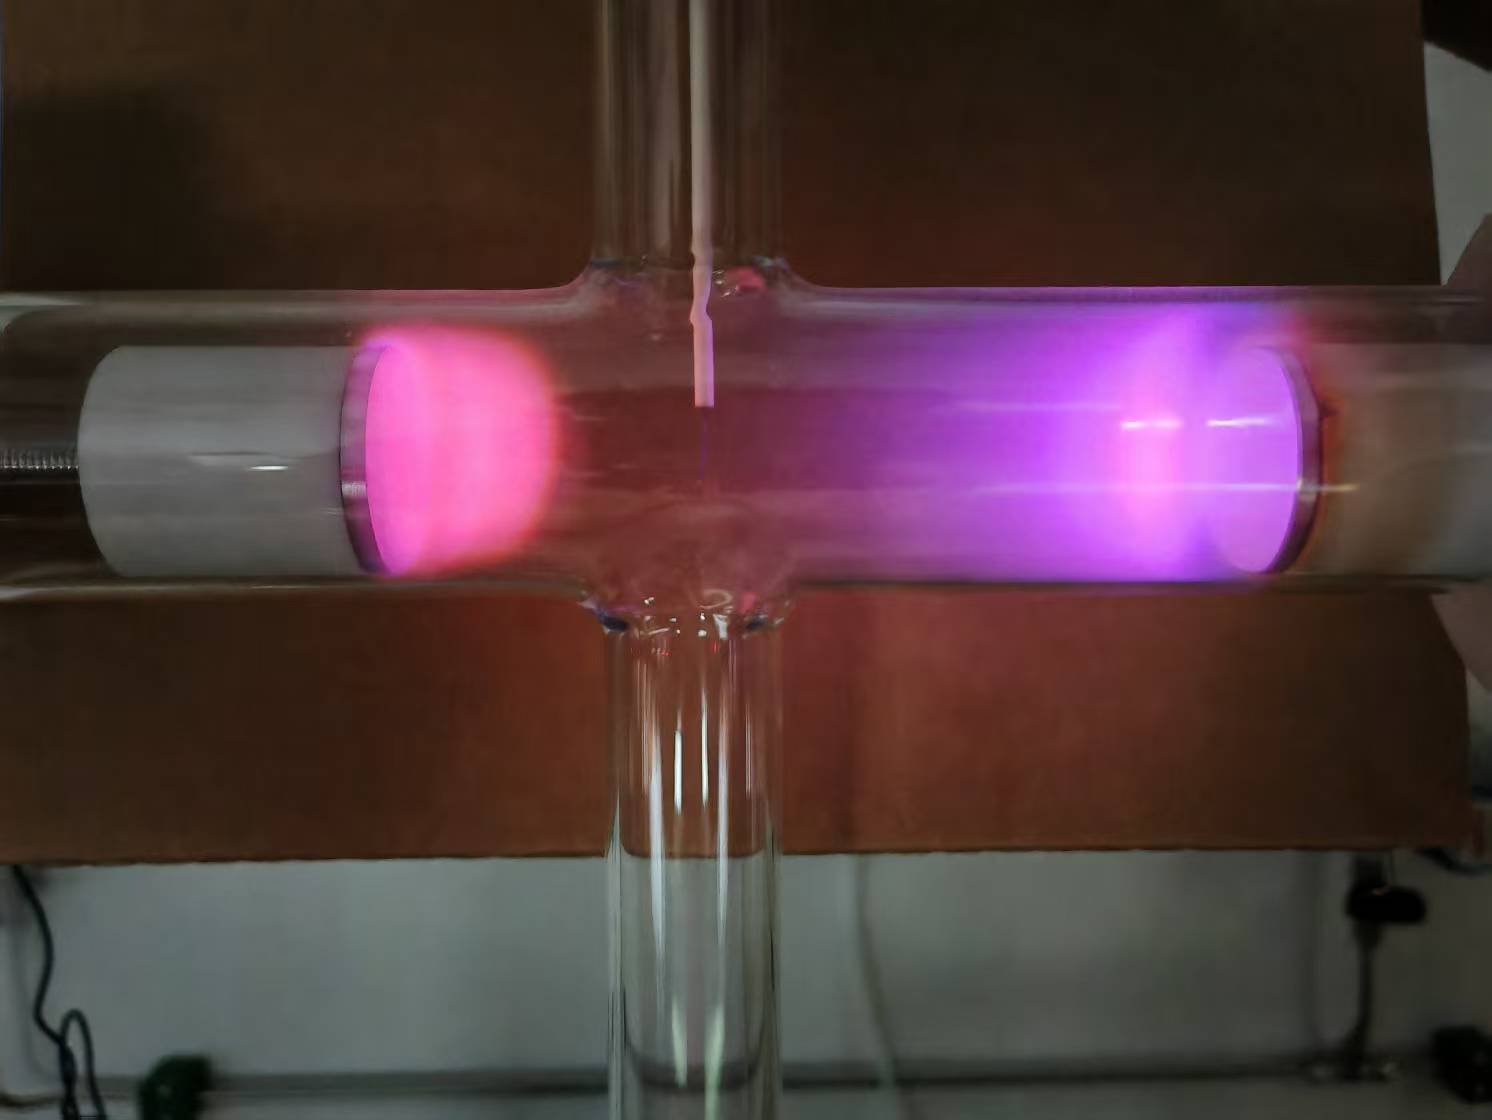
\includegraphics[width=0.3\textwidth]{20异常.jpg}
    }
    \subfloat[30Pa时的异常辉光放电]{
        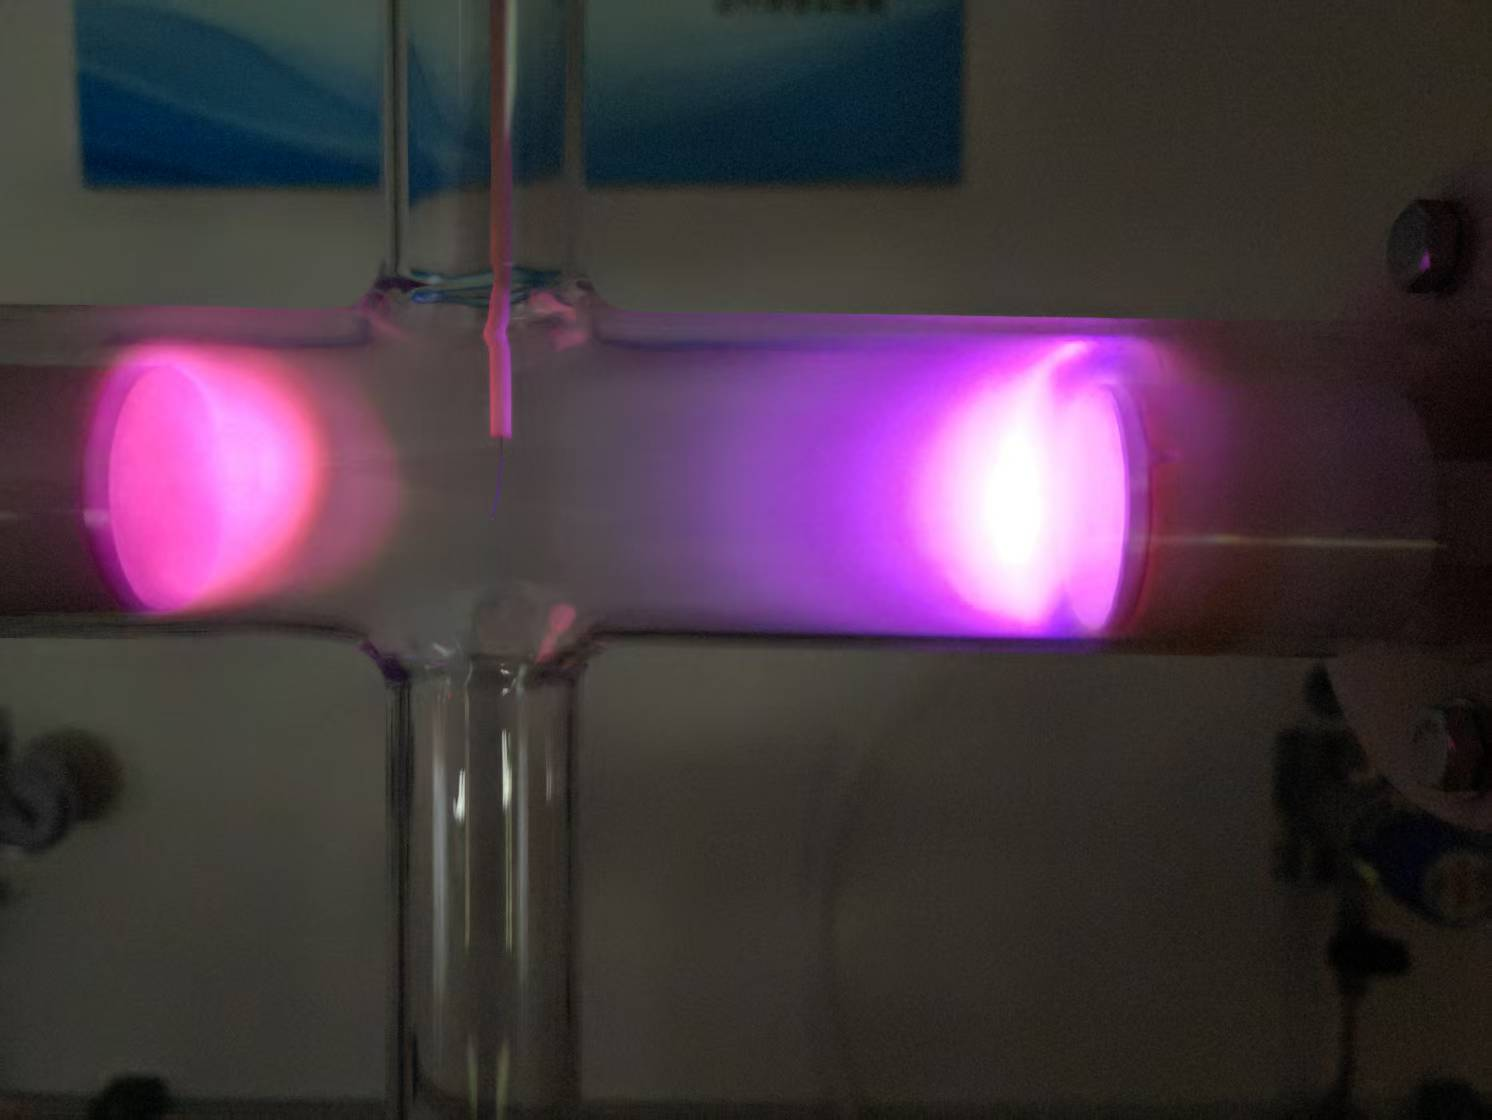
\includegraphics[width=0.3\textwidth]{30异常.jpg}
    }
    \subfloat[40Pa时的异常辉光放电]{
        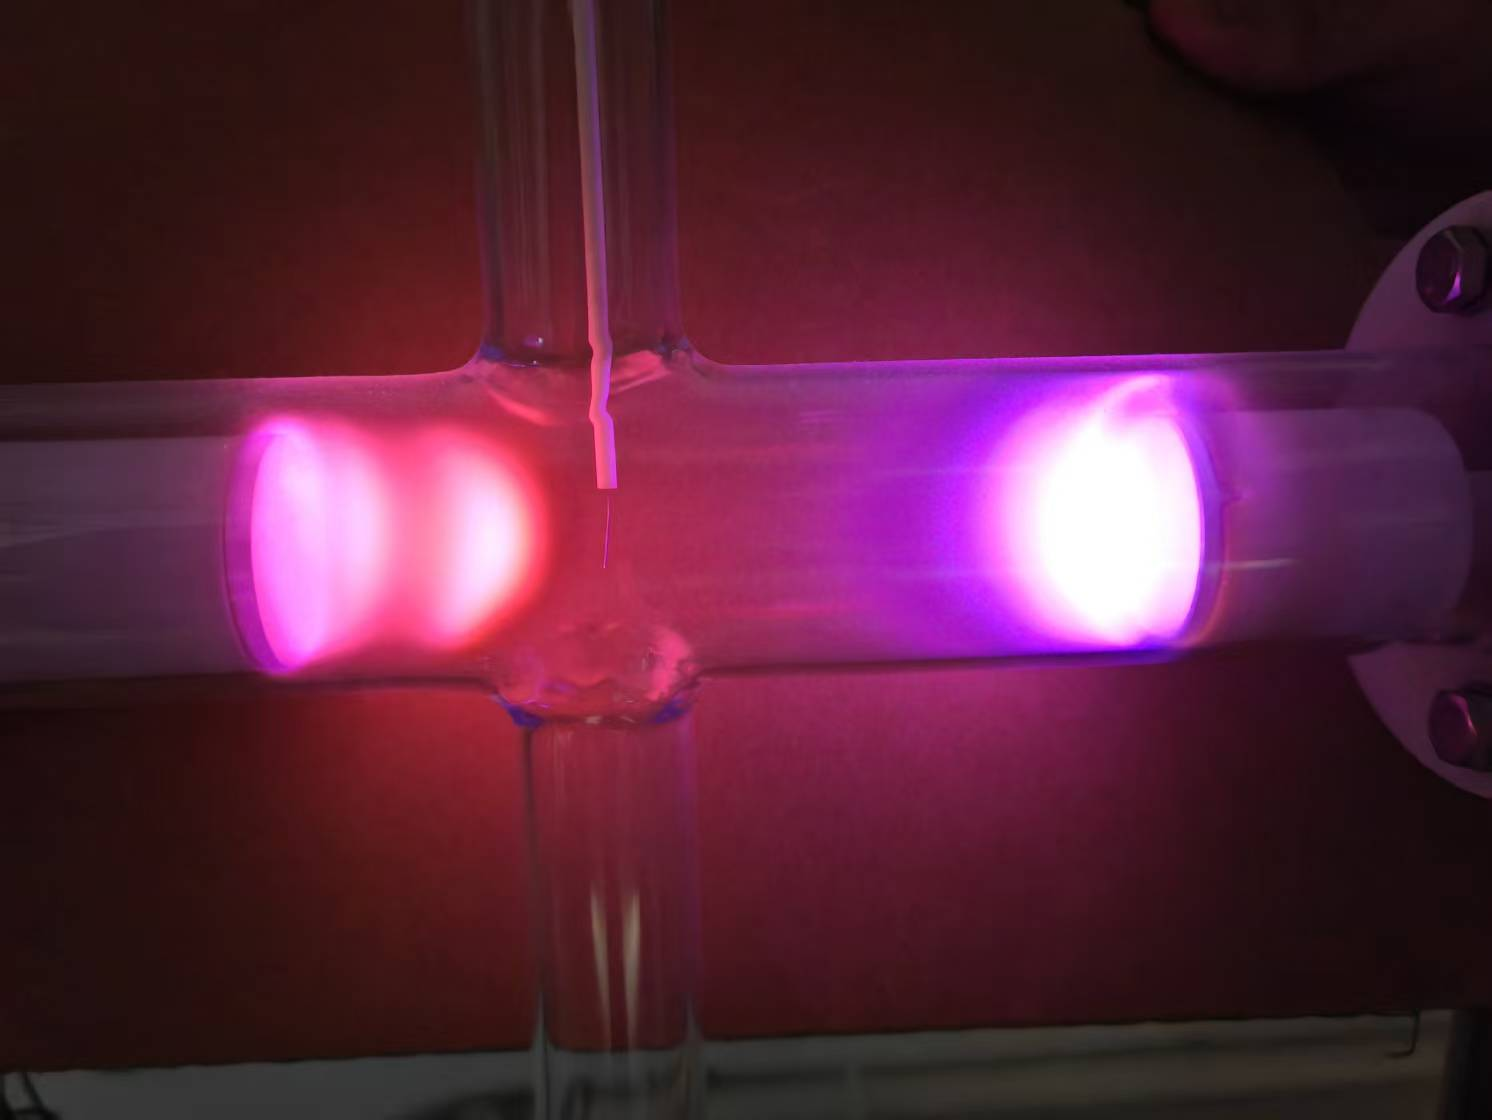
\includegraphics[width=0.3\textwidth]{40异常.jpg}
    }
    \caption{不同气压下的辉光放电现象}
    \label{fig:glow_discharge}
\end{figure}

从图\ref{fig:glow_discharge}中可以观察到，随着气压的增加，辉光放电的形态发生了明显变化。在较低气压（20Pa）时，正柱区较长且明亮；而随着气压升高，正柱区逐渐缩短，阴极辉光区与阳极辉光区的间距减小。这是因为气压升高导致气体分子密度增大，电子的平均自由程减小，从而影响了放电的空间分布特性。

\textbf{在实验的第二周进行的是等离子体诊断实验}

\subsubsection*{1.调整真空度}
这一部分的调节方法和注意事项与气体放电实验相同，这里不再赘述。

\subsubsection*{2.测量等离子体的V-I特性曲线} 
测量的操作也与气体放电实验基本相同，我们先按照气体放电实验的步骤，调节出正常辉光放电的区域，并使得朗缪尔探针位于等离子体区（即正柱区）。
随后即可开始调节探针电压，测量等离子体的I-V特性曲线。

测量得到的曲线如下：

\begin{figure}[h!]
    \centering
    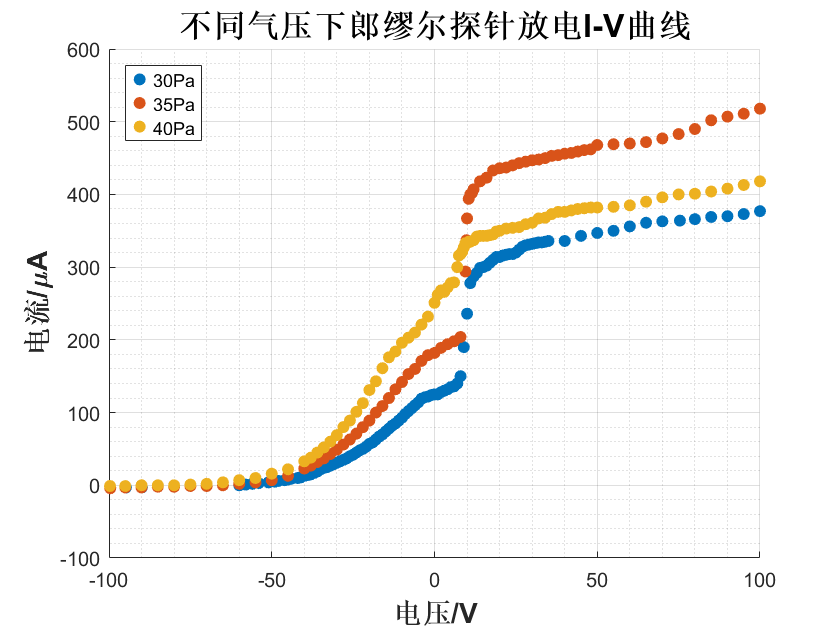
\includegraphics[width=0.8\textwidth]{DIV.png}
    \caption{等离子体的I-V特性曲线}	
\end{figure}

值得注意的是，我们发现处于过渡区的电流跳变非常剧烈，在突变区能够采集到的数据点较少。
我们将考虑在后续的实验中，使用更小的步长，或者使用更小的电压范围，来采集更多的数据点。

\subsubsection*{3.计算等离子体参数}
根据上面测量得到的曲线，我们可以读出不同气压下等离子体的悬浮电位、空间电位，结果如下表所示。

\begin{table}[h!]
    \centering
    \caption{不同气压下等离子体参数测量结果}
    \begin{tabular}{|c|c|c|}
        \hline
        \textbf{气压 (Pa)} & \textbf{悬浮电位 $V_f$ (V)} & \textbf{空间电位 $V_p$ (V)} \\
        \hline
        30 & -60 & 14 \\
        \hline
        35 & -65 & 11 \\
        \hline
        40 & -80 & 8.5 \\
        \hline
    \end{tabular}
    \label{tab:plasma_parameters}
\end{table}

根据朗缪尔探针理论，我们可以通过I-V曲线的过渡区计算电子温度。将过渡区的电流取自然对数后，绘制$\ln(I)$-$V$图，其斜率与电子温度满足关系：

\begin{equation}
    \text{slope} = \frac{e}{kT_e}
\end{equation}

通过对过渡区数据进行线性拟合，我们得到了不同气压下的斜率和对应的电子温度，结果如下表所示：

\begin{table}[h!]
    \centering
    \caption{不同气压下过渡区斜率与电子温度计算结果}
    \begin{tabular}{|c|c|c|}
        \hline
        \textbf{气压 (Pa)} & \textbf{过渡区斜率 (V$^{-1}$)} & \textbf{电子温度 $T_e$ (eV)} \\
        \hline
        30 & 0.1825 & 5.4795 \\
        \hline
        35 & 0.2409 & 4.1511 \\
        \hline
        40 & 0.5075 & 1.9704 \\
        \hline
    \end{tabular}
    \label{tab:electron_temperature}
\end{table}

从上表数据可以观察到，随着气压的增加，电子温度呈现明显的下降趋势。
当气压从30Pa增加到40Pa时，电子温度从5.48eV降低到1.97eV，降幅达到约64$\%$。
这一现象可以解释为：气压升高导致气体分子密度增大，电子与中性粒子的碰撞频率增加，电子在碰撞中损失能量的机会更多，因此平均能量（即电子温度）降低。
这与等离子体物理中的理论预期相符，即在其他条件相同的情况下，气压与电子温度通常呈负相关关系。

此外，根据电子饱和电流，我们还计算了等离子体密度：

\begin{table}[h!]
    \centering
    \caption{不同气压下等离子体密度计算结果}
    \begin{tabular}{|c|c|c|}
        \hline
        \textbf{气压 (Pa)} & \textbf{电子饱和电流 $I_{sat}$ ($\mu A$)} & \textbf{等离子体密度 $n_e$ ($\times 10^{13}$ m$^{-3}$)} \\
        \hline
        30 & 299 & 4.8614 \\
        \hline
        35 & 400 & 7.4721 \\
        \hline
        40 & 321 & 8.7035 \\
        \hline
    \end{tabular}
    \label{tab:plasma_density}
\end{table}

从上表数据可以观察到，随着气压的增加，等离子体密度呈现上升趋势。
根据讲义中的观点，我们认为三组实验中的等离子体都属于高密度等离子体，其密度量级在$10^{13}$ m$^{-3}$范围内。
当气压从30Pa增加到40Pa时，等离子体密度从$4.86 \times 10^{13}$ m$^{-3}$增加到$8.70 \times 10^{13}$ m$^{-3}$，增幅约为79$\%$。
值得注意的是，电子饱和电流在气压为35Pa时达到最大值$400\mu$A，而后在$40Pa$时略有下降至$321\mu$A。这表明电子饱和电流与气压并非简单的线性关系，可能受到多种因素的复合影响。

尽管电子饱和电流在高气压下有所下降，但等离子体密度仍然继续增加，这可能是由于电子温度的显著降低（如前文所述，从$5.48\mathrm{eV}$降至$1.97\mathrm{eV}$）导致的计算结果。
根据朗缪尔探针理论，等离子体密度与电子饱和电流和电子温度都有关系，在电子温度降低的情况下，即使电子饱和电流略有下降，计算得到的等离子体密度仍可能增加。

\subsection*{【思考题】}
本实验的实验讲义中没有给出思考题，这里我们根据实际操作实验的过程中遇到的问题和实验数据分析得到的结论，提出以下几个问题，并给出自己的🤔
\subsubsection*{1. 电流表读数波动的原因分析}
\textbf{答：}  
电流表读数的波动，既可能来源于等离子体本身的不稳定性，也可能是测量系统产生的噪声或干扰。具体物理因素和改进方法包括：  
\begin{itemize}
  \item \textbf{等离子体本身的波动}：  
  \begin{itemize}
    \item \emph{碰撞频率波动}：高气压下电子–中性分子碰撞增加，会导致局部载流子密度和温度短时波动；  
    \item \emph{电极表面发射不均匀}：阴极温度或材料微小不均一，会引起发射电流的脉动；  
    \item \emph{电晕或微小放电路径切换}：局部电场突然增强或弱化时，放电通道会改道，引起电流抖动。
  \end{itemize}
  \item \textbf{测量系统的干扰}：  
  \begin{itemize}
    \item \emph{电磁干扰}：实验室高压电源或周围仪器产生的射频干扰会叠加在微安表读数上；  
    \item \emph{接地回路}：地线不良、接地回路环路面积过大，会引入工频或射频噪声；  
    \item \emph{表内时间常数}：微安表本身或前端放大器的滤波时间常数过小，无法对快速抖动进行平滑。
  \end{itemize}
  \item \textbf{改进措施}：  
  \begin{enumerate}
    \item 在放电管与测量电路之间增加小电容（\,$\sim$10 nF）或电阻–电容低通滤波网络，降低高频波动；  
    \item 对高压电源与测量电路分别独立接地，尽量缩小接地回路面积，并在关键节点加装屏蔽罩；  
    \item 控制气压和电流稳定升降，避免快速扫压；实验中采用稳压电源并在每个数据点等待足够平衡时间（数秒）；  
    \item 如果条件允许，可使用数字示波器捕捉电流瞬时波形，并用平均值代替单点读数。
  \end{enumerate}
\end{itemize}

\subsubsection*{2. 如何改进朗缪尔探针测量方法以提高准确性？}
\textbf{答：}  
要减小探针对等离子体的扰动并提高测量精度，可从探针结构和测量流程两方面入手：
\begin{itemize}
  \item \textbf{探针设计优化}
  \begin{itemize}
    \item \emph{减小探针尺寸}：尖端直径$\ll$德拜长度，可使用直径0.05 mm以下的钨丝；  
    \item \emph{表面光滑处理}：抛光或氧化去除粗糙度和杂质，减少二次电子发射；  
    \item \emph{采用双探针或三探针技术}：可同时测量浮动电位和饱和电流，省去参考地线、减小测量误差。
  \end{itemize}
  \item \textbf{测量流程改进}
  \begin{itemize}
    \item \emph{缓慢扫描}：探针偏压以$\le$0.5 V/s的速率扫描，避免过快改变导致电容耦合误差；  
    \item \emph{多次重复测量并取平均}：在同一点重复3–5次，剔除明显异常值后平均；  
    \item \emph{温度与压力监控}：加强对气体温度、压强的实时监测与反馈，保证每次测量条件一致；  
    \item \emph{数字滤波与后处理}：对原始I–V曲线进行低通滤波或小波去噪，再做对数线性拟合。
  \end{itemize}
  \item \textbf{高气压条件下的特别注意}
  \begin{itemize}
    \item 降低探针电压扫描范围，避免出现二次放电；  
    \item 增加探针与玻璃管壁的距离，防止高压下壁面放电污染探针；  
    \item 使用等离子体或参考电极补偿法，校正电极位降引入的系统误差。
  \end{itemize}
\end{itemize}

\subsubsection*{3. 气压与放电特性的关系}
\textbf{答：}  
当气压在 $10\text{ Pa}\sim100\text{ Pa}$ 范围内变化时，放电特性主要遵循托森（Paschen）定律和碰撞理论：
\begin{itemize}
  \item \textbf{电子温度 $T_e$} 随气压升高而 \emph{逐渐降低}：  
  气压增大→中性分子密度增大→电子–中性碰撞频率提高→电子能量更快被耗散，$T_e$ 从约$3\,$eV降至$\sim1\,$eV。
  \item \textbf{等离子体密度 $n_e$} 随气压升高先 \emph{增大}，后趋于 \emph{饱和甚至下降}：  
  \begin{itemize}
    \item 在低压区（$10\text{–}30\,$Pa），碰撞电离效率上升，$n_e$ 可从$10^{15}$ m$^{-3}$增至$10^{16}$ m$^{-3}$；  
    \item 在中高压区（$30\text{–}100\,$Pa），复合和重组过程加剧，$n_e$ 增长放缓，甚至因体积复合损失略有下降。
  \end{itemize}
  \item \textbf{与理论模型的一致性}：  
  \begin{itemize}
    \item 以上趋势与 \emph{碰撞–电离平衡模型} 和 Paschen 曲线预测相符：最低点附近的分压–距离乘积最易放电；  
    \item 在超出实验管长或电极间距范围时，可能出现“放电难起火”或“过渡到异常辉光／弧光”现象，与理论略有偏差，需要考虑壁面效应和电子附着。
  \end{itemize}
\end{itemize}


\bibliography{ref.bib} %biblatex -> 'xelatex->pdfletax->xelatex'
\bibliographystyle{ieeetr}

\subsection*{【原始数据的记录】}
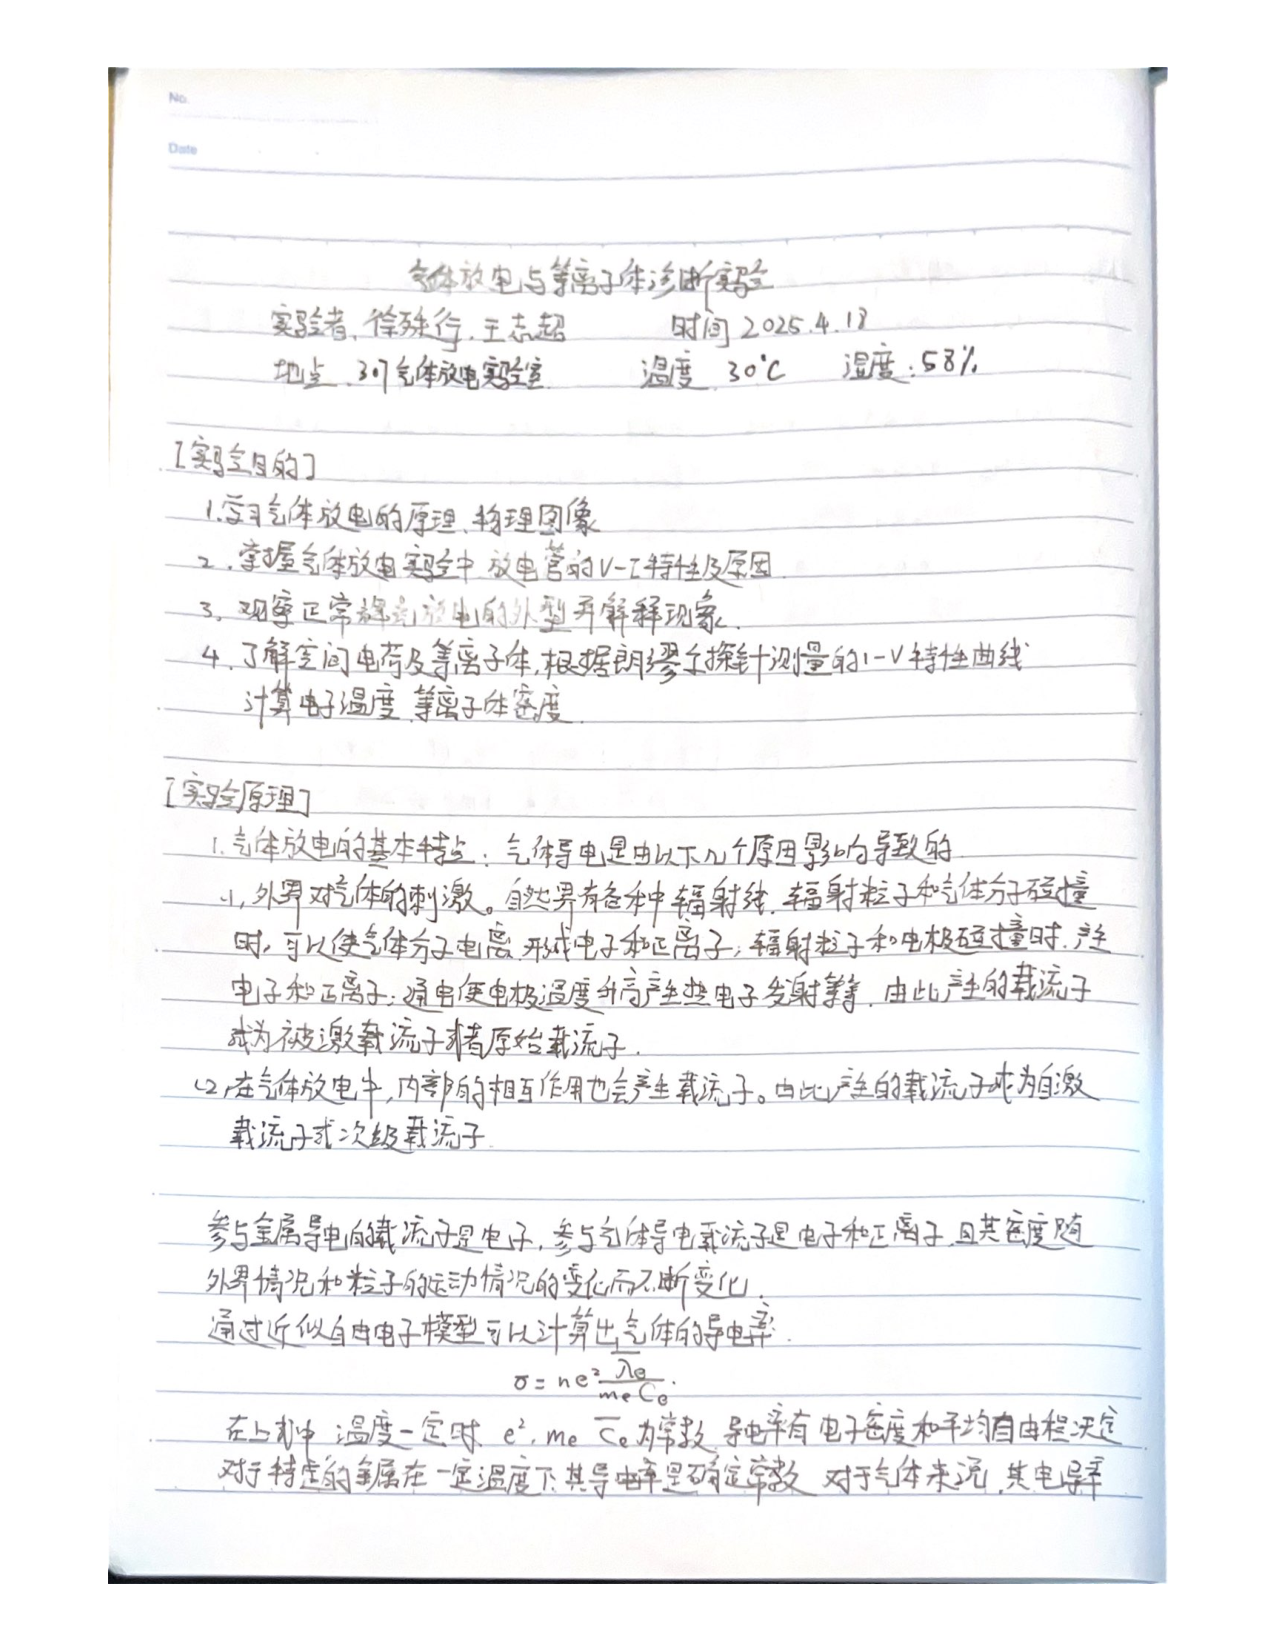
\includepdf[pages=-]{气体放电scan.pdf}

\end{document}

